%=====================================================================
\chapter{Decision-Theoretic Allocation and Cross-Market Validation}
\label{ch:allocation}
%=====================================================================

\textbf{Research Objective 4.} \emph{To evaluate and validate the result and practical
application of the proposed model across different stock markets, exploring transfer learning
techniques for cross-market applications and validating the model against benchmark datasets and
real-world market data.}

\vspace{0.4em}
This chapter converts a fused signal into an executable portfolio and then takes the framework
apart to determine which of its layers produces the measured outcome. The second half of that
sentence is the contribution. It is straightforward to build an allocation framework that beats a
benchmark on a backtest; it is considerably harder to establish \emph{why} it beat the benchmark,
and the answer obtained here is not the answer the design anticipated.

Section~\ref{sec:alloc-design} specifies the framework, Section~\ref{sec:alloc-setup} the data and
protocol, and Section~\ref{sec:alloc-defects} documents two implementation defects that had
silently invalidated an earlier version of this study --- both of which produce no error message
and both of which generalise well beyond this framework. Sections~\ref{sec:alloc-main}
to~\ref{sec:alloc-sig} report the evidence, Section~\ref{sec:alloc-transfer} the cross-market
test, and Section~\ref{sec:alloc-limits} the limits.

The work reported in this chapter appears in publication~\pubcite{P5}; supporting sectoral and
regime-level evidence comes from~\pubcite{P1} and~\pubcite{P2}.

\section{Design of the Decision-Theoretic Allocation Framework}
\label{sec:alloc-design}

\subsection{The separation principle}

The framework is built around one architectural decision from which everything else follows: the
allocation problem is separated into two questions that are answered by different mechanisms.

\begin{itemize}
\item \textbf{Relative composition:} what to hold relative to everything else. This is answered by
a constrained quadratic program over the risky sleeve.
\item \textbf{Total risk:} how much of the portfolio to expose to that sleeve at all. This is
answered by a regime-dependent risk budget, with the residual held in cash.
\end{itemize}

The separation is not a presentational convenience. It is what makes the framework
\emph{falsifiable layer by layer}. Because composition and risk level are produced by distinct
mechanisms, either can be disabled while the other is held fixed, and --- crucially --- a control
can be constructed that carries the same \emph{average} exposure as the full framework but
allocates it without regard to the regime. The difference between the framework and that control
isolates the \emph{timing} of risk from its \emph{level}. Without the separation, that experiment
cannot be constructed at all, and Section~\ref{sec:alloc-ablation} is the return on the design
decision.

\subsection{Stage 1: cross-sectional feature construction}

Nine causal features are computed per asset per session and standardised
\emph{cross-sectionally} into two composites: a technical composite $T_{i,t}$ and a sentiment
composite $M_{i,t}$.

Cross-sectional rather than time-series standardisation is deliberate and has two effects. A
standardised value expresses how an asset ranks against its peers \emph{on that day} rather than
against its own history, which is the relevant comparison for a cross-sectional allocation. And it
removes the common market factor: when every asset rises together, every raw indicator moves
together, and a time-series standardisation would register a signal on every asset simultaneously
--- which is not a cross-sectional signal at all but a disguised market-timing bet.

\subsection{Stage 2a: regime identification}

The market state $r_t$ is identified by a three-component Gaussian mixture over a two-dimensional
feature vector of rolling realised volatility and rolling momentum, following Section~2.7.2. Two
protocol requirements apply and both are load-bearing.

The mixture is \textbf{refitted at every rebalance} on an expanding window of strictly earlier
sessions. Fitting once on the full sample and labelling the history backwards would let the
identification of ``stress'' be informed by knowing when stress occurred.

The components are \textbf{anchored by ascending fitted volatility} into calm, transitional and
stress states. Expectation maximisation returns component indices in arbitrary order that permute
freely between refits, so without anchoring, component~0 in one refit need not correspond to
component~0 in the next. The failure mode is silent: no error is raised, and the downstream results
look entirely plausible while resting on a scrambled state series.

\subsection{Stage 2b: signal fusion and scaling}

The two composites are fused with state-dependent weights and a confidence term $c_{i,t}$ that
discounts assets whose composites disagree,
\begin{equation}
z_{i,t} = c_{i,t}\left(w^{T}_{r_t}\, T_{i,t} + w^{M}_{r_t}\, M_{i,t}\right),
\label{eq:alloc-fuse}
\end{equation}
and the fused score is placed on a return scale by information-ratio
scaling~\cite{grinold2000},
\begin{equation}
\alpha_{i,t} = \mathrm{IC}\cdot\sigma_{i,t}\cdot z_{i,t}.
\label{eq:alloc-scale}
\end{equation}
The state dependence in Equation~\eqref{eq:alloc-fuse} encodes the hypothesis that the relative
informativeness of the two composites varies with the market state --- specifically, that
sentiment becomes relatively more informative under stress. Section~\ref{sec:alloc-ic} tests that
hypothesis directly and does not find support for it.

Equation~\eqref{eq:alloc-scale} is not cosmetic, for reasons Section~\ref{sec:alloc-defects}
makes concrete.

\subsection{Stage 3a: relative composition}

The risky sleeve is obtained by solving
\begin{equation}
\tilde{w}_t = \arg\max_{w}\;
\alpha_t^{\!\top} w \;-\; \lambda\, w^{\!\top}\Sigma_t w \;-\; \kappa\left\|w - w_{t-1}\right\|_1
\quad\text{s.t.}\quad
w \ge 0,\;\; w \le 0.25,\;\; \mathbf{1}^{\!\top} w = 1,
\label{eq:alloc-qp}
\end{equation}
where $\Sigma_t$ is estimated by Ledoit--Wolf shrinkage~\cite{ledoit2004}, the position cap of 25
per cent limits concentration, the long-only constraint reflects the scope delimitation of
Section~1.7, and the turnover penalty $\kappa$ annualises a one-way transaction cost of ten basis
points so that the optimiser trades only when the expected gain exceeds the cost of trading.

\subsection{Stage 3b: total risk}

The sleeve is then scaled by the regime risk budget,
\begin{equation}
w_t^{*} = k_{r_t}\,\tilde{w}_t,
\qquad
k = \{1.00,\ 0.75,\ 0.50\}\ \text{for calm, transitional and stress states},
\label{eq:alloc-budget}
\end{equation}
with the residual $1 - k_{r_t}$ held in cash. Two properties of
Equation~\eqref{eq:alloc-budget} matter.

The budget is expressed as a \emph{fraction of the sleeve's own volatility} rather than as an
absolute annualised target. Section~\ref{sec:alloc-defects} documents what happens when it is not.

The scaling is \emph{one-sided}: $k \le 1$ always, so the framework de-risks toward cash in
disturbed states but never levers up. This guarantees that any measured performance difference
against a fully invested benchmark is attributable to risk \emph{reduction} rather than to
leverage, which removes an entire class of alternative explanations before the evaluation begins.

\subsection{Stage 4: evaluation and ablation}

The evaluation applies a 21-session walk-forward with ten basis points of transaction costs, an
18-cell specification sweep, matched-exposure ablation, four pre-selected stress episodes, a
665-session holdout postdating every design decision, and a secondary market universe, with
Newey--West~\cite{newey1987} and stationary block bootstrap~\cite{politis1994} inference.

\section{Data and Experimental Protocol}
\label{sec:alloc-setup}

\subsection{Universes}

The \textbf{primary universe} is ten liquid multi-asset exchange-traded instruments spanning
United States large capitalisation, technology-weighted large capitalisation, small
capitalisation, developed international equity, emerging-market equity, long-duration and
intermediate-duration government bonds, investment-grade credit, gold and real estate. The
\textbf{secondary universe}, used as a cross-market test, is ten mega-capitalisation United States
equities over 2019--2026.

The choice of universe requires justification, because this thesis is otherwise centred on the
Indian market. Two requirements bind. The allocation study needs eighteen years of clean,
survivorship-free daily history including at least two severe crises, because a claim about
drawdown behaviour cannot be made on a sample containing no drawdowns. And it needs genuine
dispersion in asset volatility, because a regime-conditional risk budget that de-risks into cash
has nothing to rotate toward in a universe where every instrument carries similar risk. The
instruments satisfying both requirements are the multi-asset exchange-traded funds used here. The
study is therefore conducted as a test of the \emph{mechanism} rather than as a claim about Indian
allocation, and Section~\ref{sec:alloc-transfer} reports what happens when the transferability
condition is violated. Complementary evidence at sectoral granularity on the Indian market comes
from the ten-sector evaluation of Chapter~\ref{ch:fusion} and the regime-level behaviour of
Chapter~\ref{ch:causal}.

\subsection{Period, protocol and benchmarks}

The primary sample runs from January 2008 to August 2026, comprising 4,689 trading sessions, with
rebalancing every 21 sessions --- 224 rebalance dates in total. Table~\ref{tab:alloc-spec} records
the full specification.

\begin{table}[!htb]
\centering
\caption[Specification of the allocation framework]{Complete specification of the reported
allocation framework configuration}
\label{tab:alloc-spec}
\tabfont
\begin{tabular}{@{}L{5.2cm}L{4.0cm}L{4.6cm}@{}}
\toprule
\textbf{Parameter} & \textbf{Value} & \textbf{Basis} \\
\midrule
Primary universe & 10 multi-asset instruments & Volatility dispersion and clean history \\
Sample & Jan 2008 -- Aug 2026, 4,689 sessions & Includes 2008 and 2020 crises \\
Rebalance interval & 21 sessions (224 rebalances) & Monthly; swept over $\{10, 21, 42\}$ \\
Covariance lookback & 252 sessions & Swept over $\{126, 252\}$ \\
Covariance estimator & Ledoit--Wolf shrinkage & Conditioning on 10 assets \\
Transaction cost & 10\,bp one way & Charged to the strategy only \\
Position cap & 25\% & Concentration limit \\
Risk aversion $\lambda$ & 2.0 & Fixed \emph{a priori} \\
Assumed information coefficient & 0.05 & Conservative; scaling only \\
Number of regimes $K$ & 3 & Calm / transitional / stress \\
Regime multipliers $k$ & $\{1.00, 0.75, 0.50\}$ & Fixed \emph{a priori}, one-sided \\
Random seed & 42 & Swept over $\{0, 7, 42\}$ \\
\bottomrule
\end{tabular}
\end{table}

Three benchmarks are used. \textbf{Equal weight} is the primary benchmark, following DeMiguel et
al.~\cite{demiguel2009}: a framework that cannot beat $1/N$ has not earned its complexity.
\textbf{Inverse volatility} is a stronger risk-based competitor. \textbf{Equal weight at strategy
volatility} scales the equal-weight portfolio to the same realised volatility as the framework,
which is the fair comparison for a Sharpe ratio.

All three benchmarks are rebalanced daily and charged \emph{no} transaction costs, while the
framework pays ten basis points on every trade. This is deliberately unfavourable to the framework
and is stated so that the reported margins are read as conservative.

\section{Two Silent Implementation Defects}
\label{sec:alloc-defects}

Before the results, two defects are documented that had invalidated an earlier version of this
study. Both were found only by disassembling the framework to construct the robustness analysis;
both produce no error message; and both generalise well beyond this work. They are reported here
rather than buried because the corrected framework cannot be understood without them, and because
the class of failure they represent is under-reported in the literature.

\subsection{Scale mismatch in signal-to-allocation conversion}

In the defective version, the fused signal entered the quadratic program of
Equation~\eqref{eq:alloc-qp} in \emph{raw indicator units}. Among the nine causal features is an
on-balance volume accumulator, which on liquid instruments takes values of order $10^{8}$ to
$10^{9}$. The risk term $\lambda w^{\!\top}\Sigma_t w$ is of order $10^{-4}$.

The consequence is that the linear term dominated the quadratic term by twelve orders of
magnitude, so the covariance matrix was effectively irrelevant to the solution. The optimiser
placed the entire budget on whichever asset had the largest raw signal, subject only to the
position cap, on almost every rebalance date. The reported behaviour of the framework was therefore
determined by the \emph{ratio of measurement units} between the two terms of the objective, not by
any information in the signal.

Nothing in the code failed. The optimiser converged, the constraints were satisfied, the backtest
ran, and the resulting equity curve was plausible enough to be published. The remedy is
Equation~\eqref{eq:alloc-scale}: information-ratio scaling places the signal on a return metric so
that the two terms of the objective are commensurable, and the risk model resumes doing work.

The general lesson is worth stating independently of this framework. Whenever a signal enters a
mean-variance objective, the units of the linear and quadratic terms must be reconciled
explicitly. A concentrated, nearly single-asset solution on almost every date is the diagnostic
symptom.

\subsection{An inert risk layer}

In the same defective version, the regime risk budget was specified as \emph{absolute} annualised
volatility targets of 20, 15 and 10 per cent for the three states. The risky sleeve of a
diversified ten-instrument multi-asset portfolio carries a realised volatility of about 6.4 per
cent.

An absolute target binds only when the portfolio's own volatility exceeds it. At 6.4 per cent
against a floor of 10 per cent, the target bound in \textbf{one rebalance out of 224}. The regime
layer --- the central mechanism of the framework --- was present in the specification, consumed
computation at every rebalance, and did nothing on 223 of 224 occasions.

Again nothing failed. The regime model fitted, the states were identified, the multipliers were
computed, and the results were reported as though the layer had been active. The remedy is
Equation~\eqref{eq:alloc-budget}: expressing the budget as a \emph{fraction of the sleeve's own
volatility} makes it scale-free, so it remains active in any universe.

The general lesson is that an absolute volatility target is not scale-free, and moving a strategy
between universes can therefore disable it silently. Any risk layer should be instrumented with a
count of how often it actually binds --- a one-line diagnostic that would have caught this
immediately.

\section{Main Results}
\label{sec:alloc-main}

Table~\ref{tab:port} consolidates the evaluation across the primary universe, the holdout, the
specification sweep and the secondary market.

\begin{table}[!htb]
\centering
\caption[Portfolio-level evaluation across universes and periods]{Portfolio-level evaluation.
Benchmarks are rebalanced daily and charged no transaction costs, which is deliberately
unfavourable to the proposed framework.}
\label{tab:port}
\tabfont
\begin{tabular}{@{}L{5.0cm}rrrrr@{}}
\toprule
\textbf{Configuration} & \textbf{CAGR} & \textbf{Vol.} & \textbf{Sharpe} &
\textbf{Max DD} & \textbf{Calmar} \\
\midrule
\multicolumn{6}{@{}l@{}}{\textit{Primary universe: ten multi-asset instruments, Jan 2008 -- Aug
2026, 4{,}689 sessions}}\\
Proposed regime-conditional framework & 5.65\% & 6.44\% & \textbf{0.878} &
\textbf{$-$18.98\%} & 0.298 \\
Equal-weight benchmark & 8.45\% & 13.45\% & 0.628 & $-$36.08\% & 0.234 \\
Inverse-volatility benchmark & 7.46\% & 8.78\% & 0.849 & $-$24.09\% & 0.310 \\
Equal-weight at strategy volatility & 4.19\% & 6.44\% & 0.651 & $-$18.69\% & 0.224 \\
\midrule
\multicolumn{6}{@{}l@{}}{\textit{Out-of-sample holdout: 665 sessions, Jan 2024 -- Aug 2026}}\\
Proposed framework & 12.32\% & 7.63\% & \textbf{1.614} & \textbf{$-$5.48\%} & 2.246 \\
Equal-weight benchmark & 15.44\% & 11.10\% & 1.391 & $-$10.13\% & 1.524 \\
Inverse-volatility benchmark & 11.89\% & 8.51\% & 1.397 & $-$6.70\% & 1.775 \\
Equal-weight at strategy volatility & 7.28\% & 5.32\% & 1.370 & $-$7.04\% & 1.473 \\
\midrule
\multicolumn{6}{@{}l@{}}{\textit{Specification sweep: 3 seeds $\times$ 2 covariance windows
$\times$ 3 rebalance intervals}}\\
Range across all 18 cells & --- & --- & 0.813 -- 0.956 & $-$21.1\% -- $-$19.0\% & --- \\
Cells beating the benchmark on both measures & \multicolumn{5}{l}{18 of 18} \\
\midrule
\multicolumn{6}{@{}l@{}}{\textit{Secondary universe: ten mega-capitalisation equities, 2019 --
2026 (cross-market transfer)}}\\
Proposed framework & 17.02\% & 14.87\% & 1.145 & \textbf{$-$20.45\%} & 0.832 \\
Equal-weight benchmark & 33.52\% & 24.45\% & \textbf{1.371} & $-$33.63\% & 0.997 \\
\bottomrule
\end{tabular}
\end{table}

\subsection{The primary universe}

On the primary universe the framework raises the Sharpe ratio from 0.628 to 0.878, a gain of 40
per cent, and reduces maximum drawdown from $-36.08$ to $-18.98$ per cent, a reduction of 47 per
cent, while earning a lower compound return of 5.65 against 8.45 per cent per annum.

The correct characterisation is therefore a \emph{risk-reduction instrument whose return sacrifice
is smaller than its risk reduction}, and it is presented as such rather than as a
return-enhancing one. An investor unwilling to give up return should not deploy it.

Against the volatility-matched benchmark the reading is more precise and less flattering. The
framework retains its Sharpe advantage --- 0.878 against 0.651 --- but loses marginally on
drawdown, $-18.98$ against $-18.69$ per cent. This bounds the drawdown claim exactly: the
framework reduces drawdown relative to an unlevered diversified benchmark, \emph{not} relative to
every portfolio held at the same volatility. Stating the bound is what makes the unbounded version
of the claim unnecessary.

\subsection{The holdout}

The holdout block is the single strongest piece of evidence in this thesis, and the reason is
procedural rather than statistical. Every specification decision --- universe, feature set, number
of regimes, risk budget multipliers, rebalancing interval, cost assumption --- was fixed before any
session in the holdout was examined. The 665 sessions from January 2024 postdate the entire design.

On those sessions the framework records a higher Sharpe ratio and a smaller drawdown than all
three benchmarks, and two of those comparisons \emph{reverse} the in-sample ordering: the
inverse-volatility benchmark beats the framework on Calmar in sample and does not in the holdout.
Figure~\ref{fig:holdout} shows the comparison.

\begin{figure}[!htb]
\centering
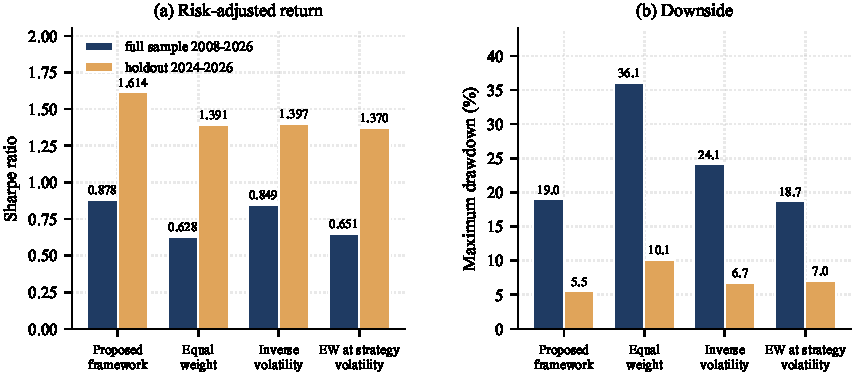
\includegraphics[width=0.98\linewidth]{figs/f_holdout.pdf}
\caption[Full-sample and holdout performance against three benchmarks]{Full-sample and holdout
performance against the three benchmarks. Every specification decision was fixed before any
holdout session was examined.}
\label{fig:holdout}
\end{figure}

Three qualifications are stated alongside, and they are not perfunctory. Six hundred and
sixty-five sessions cannot settle the question on their own. The period contains no episode
comparable to 2008 or 2020, so the holdout does not test the drawdown mechanism where it matters
most. And the framework again earns less in absolute terms than the benchmark it beats on
risk-adjusted measures.

\subsection{The specification sweep}

Reporting the best cell of a grid and omitting the grid is a misstatement of evidence, for the
reasons given in Section~2.11.3. The entire sweep is therefore reported:
three seeds $\times$ two covariance lookback windows $\times$ three rebalance intervals, eighteen
cells. Figure~\ref{fig:sweep} plots all of them.

\begin{figure}[!htb]
\centering
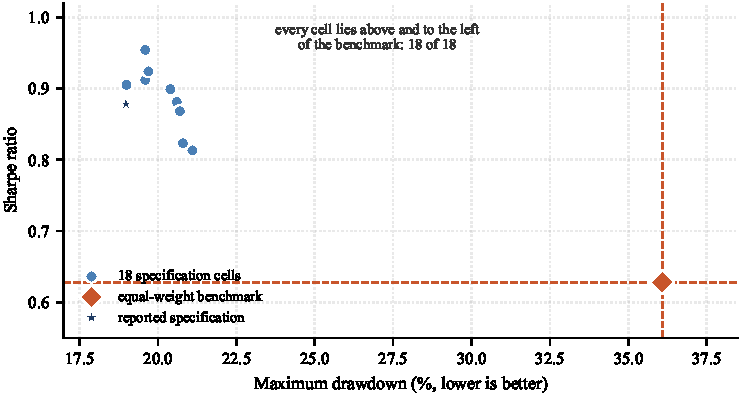
\includegraphics[width=0.84\linewidth]{figs/f_spec_sweep.pdf}
\caption[All eighteen cells of the specification sweep]{All eighteen cells of the specification
sweep on the primary universe, plotted against the equal-weight benchmark. Every cell lies above
and to the left of the benchmark, that is, higher Sharpe ratio and smaller drawdown.}
\label{fig:sweep}
\end{figure}

Sharpe ratios range from 0.813 to 0.956 and maximum drawdowns from $-21.1$ to $-19.0$ per cent.
All eighteen cells beat the equal-weight benchmark on \emph{both} measures. The reported
specification, at Sharpe 0.878, sits near the middle of that range rather than at its top --- which
is the honest position to report from and is itself informative, since a headline drawn from the
best cell would have overstated the framework by roughly nine per cent of Sharpe ratio.

\section{Component Ablation at Matched Exposure}
\label{sec:alloc-ablation}

This section contains the central result of the chapter, and the instrument that produces it is
the matched-exposure control described in Section~2.10.4.

\subsection{The control}

Comparing a de-risked framework against a fully invested benchmark confounds two effects: the
framework holds \emph{less} risk on average, and it holds risk at \emph{different times}. The
first alone will improve a drawdown statistic without any skill in timing whatever. The control
therefore carries the same average invested exposure as the full framework --- measured at 92.1
per cent --- but allocates it \emph{uniformly} rather than by regime. Any difference between the
framework and this control is attributable to the timing of risk alone.

\begin{figure}[!htb]
\centering

\includegraphics[width=0.98\linewidth]{figs/f_ablation.pdf}
\caption[Component ablation and stress-episode behaviour]{(a) Component ablation. The
matched-exposure control carries the same average invested exposure as the full framework but
applies it without regard to the regime, so that only the timing of risk differs. (b) Cumulative
advantage over the benchmark in four stress episodes chosen on documented market history, plus the
deepest benchmark drawdown in the holdout.}
\label{fig:abl}
\end{figure}

\subsection{Regime-conditional risk timing works}

Holding average exposure fixed at 92.1 per cent, allocating that exposure according to the
identified regime rather than uniformly raises the Sharpe ratio from 0.795 to 0.878 and improves
maximum drawdown from $-22.26$ to $-18.98$ per cent, with \emph{no significant difference in mean
return} ($p = 0.695$).

That combination is the signature of a genuine risk-timing effect. Both risk-adjusted measures
improve while mean return is statistically unchanged, which is what one expects if the framework is
rearranging \emph{when} it carries risk rather than simply carrying less of it. Had the mechanism
been merely holding less, mean return would have fallen measurably.

The cost of that timing is also measured, because a mechanism that improves risk-adjusted return
is not free. Against a fully invested variant, the framework gives up approximately 1.3 percentage
points of annual return, significantly so ($p = 0.016$), in exchange for 3.55 percentage points of
maximum drawdown. That is the actual trade a practitioner is being offered, and it is stated in
those terms.

\subsection{The signal fusion layer returns a null}

The same ablation removes the signal fusion layer entirely, so that the objective of
Equation~\eqref{eq:alloc-qp} reduces to a constrained minimum-variance problem. The Sharpe ratio
moves from 0.878 to 0.908 and maximum drawdown from $-18.98$ to $-18.87$ per cent. \emph{Both
movements favour removal}, and neither is significant ($p = 0.650$).

The signal fusion layer --- the component that a reader of Chapters~\ref{ch:fusion}
to~\ref{ch:causal} would expect to be central --- contributes nothing detectable to
cross-sectional selection in this framework on this universe.

This null is retained in full rather than removed, for two reasons. The first is that it is what
the evidence shows. The second is methodological: component-level negative results are rarely
published, which is one reason architectures in this literature accumulate layers whose
contribution has never been isolated. Reporting which layer works is more useful to a subsequent
researcher than an aggregate number that conceals the distinction, and a framework whose useless
component has been identified is a better engineering artefact than one whose aggregate
performance is slightly higher for unknown reasons.

\section{Why the Signal Layer Fails: Information Coefficients}
\label{sec:alloc-ic}

The ablation establishes \emph{that} the signal layer adds nothing. The information coefficients
establish \emph{why}. Table~\ref{tab:ic} and Figure~\ref{fig:ic} report them.

\begin{table}[!htb]
\centering
\caption[Cross-sectional information coefficients]{Cross-sectional information coefficients of
each composite against next-session returns, with Newey--West $t$ statistics}
\label{tab:ic}
\tabfont
\begin{tabular}{@{}L{4.2cm}rrrrrr@{}}
\toprule
& \multicolumn{2}{c}{\textbf{Technical}} & \multicolumn{2}{c}{\textbf{Sentiment}} &
\multicolumn{2}{c}{\textbf{Fused}} \\
\cmidrule(lr){2-3}\cmidrule(lr){4-5}\cmidrule(lr){6-7}
\textbf{Universe} & \textbf{IC} & \textbf{$t$} & \textbf{IC} & \textbf{$t$} & \textbf{IC} &
\textbf{$t$} \\
\midrule
Multi-asset, 2008--2026 & $-0.030$ & $-2.14$ & $-0.026$ & $-2.26$ & $-0.033$ & $-2.42$ \\
Sector rotation, 2008--2026 & $-0.007$ & $-0.49$ & $-0.008$ & $-0.62$ & $-0.005$ & $-0.37$ \\
Mega-capitalisation, 2019--2026 & $+0.035$ & $+1.52$ & $+0.029$ & $+1.51$ & $+0.044$ & $+2.02$ \\
\bottomrule
\end{tabular}
\end{table}

\begin{figure}[!htb]
\centering
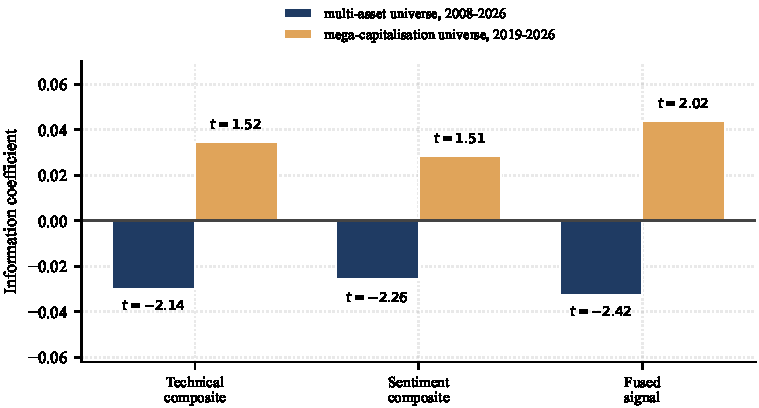
\includegraphics[width=0.84\linewidth]{figs/f_ic.pdf}
\caption[Information coefficients by universe]{Cross-sectional information coefficients of the
technical, sentiment and fused composites against next-session returns, on the primary multi-asset
universe and on the secondary mega-capitalisation universe, with Newey--West $t$ statistics.}
\label{fig:ic}
\end{figure}

Three findings follow.

\textbf{The composites are significantly negatively related to next-session returns on the primary
universe.} All three information coefficients are negative and all three carry Newey--West $t$
statistics beyond $-2$. A signal that is significantly negatively related to the target is
information, in principle; a long-only optimiser that treats it as positive will allocate away from
the assets it should hold.

\textbf{The state-dependent weighting hypothesis is not supported.} Equation~\eqref{eq:alloc-fuse}
encodes the hypothesis that sentiment becomes relatively more informative under stress. Measured
directly, the point estimates run the \emph{other way}, and the calm-to-stress contrast is
insignificant ($t = -1.46$, $p = 0.145$). The mechanism was built on a hypothesis the data do not
support, and saying so is more useful than retaining the layer on the grounds that it does no
visible harm.

\textbf{The relationship is not stable enough to exploit by inversion.} The obvious response to a
significantly negative information coefficient is to invert the signal. The sub-period breakdown
forecloses that: the coefficient is $-0.039$ before 2024 and $+0.009$ afterwards. A sign that flips
between sub-periods is not a tradable relationship; it is an in-sample artefact that inversion
would have converted into an out-of-sample loss.

The sector-rotation row is included because it is the closest available analogue to a sectoral
Indian deployment, and there the coefficients are indistinguishable from zero in either direction.
The mega-capitalisation row is positive and marginally significant on the fused signal, which is
consistent with a genuine but small cross-sectional signal existing in a universe of
heavily-researched single names and not in a universe of broad index instruments --- exactly the
structural argument of Section~3.2.3 about where instrument-level information exists.

\section{Behaviour Under Stress}
\label{sec:alloc-stress}

Four stress episodes were selected \emph{before} the analysis on documented market history rather
than by inspection of results: the global financial crisis of 2008--09, the euro area crisis of
2011, the COVID-19 crash of 2020 and the inflation-driven bear market of 2022. The deepest
benchmark drawdown within the holdout period is reported alongside as a fifth, out-of-sample
episode.

The framework outperforms in \emph{all four} pre-selected episodes, by margins between 7.73 and
22.74 percentage points, and by a further 5.42 points in the holdout drawdown
(Figure~\ref{fig:abl}(b)). Table~\ref{tab:tail} reports two complementary tail diagnostics.

\begin{table}[!htb]
\centering
\caption[Tail behaviour and capture ratios]{Tail behaviour on the primary universe: mean return on
the worst five per cent of benchmark sessions, and directional capture ratios}
\label{tab:tail}
\tabfont
\begin{tabular}{@{}L{6.0cm}rrL{3.9cm}@{}}
\toprule
\textbf{Measure} & \textbf{Framework} & \textbf{Benchmark} & \textbf{Reading} \\
\midrule
Mean return on worst 5\% of benchmark sessions & $-0.59\%$ & $-2.01\%$ & Cushion of 1.42
percentage points per session \\
Downside capture & 0.38 & 1.00 & Participates in 38\% of benchmark declines \\
Upside capture & 0.41 & 1.00 & Participates in 41\% of benchmark advances \\
Capture ratio (up/down) & 0.93 & 1.00 & Below one: no directional skill \\
\bottomrule
\end{tabular}
\end{table}

\begin{figure}[!htb]
\centering
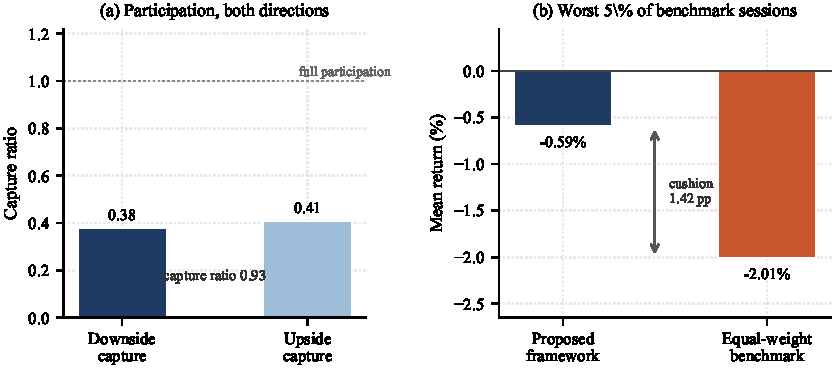
\includegraphics[width=0.92\linewidth]{figs/f_capture.pdf}
\caption[Capture ratios and tail cushion]{(a) Downside and upside capture against the benchmark.
(b) Mean return on the worst five per cent of benchmark sessions. The framework participates less
in both directions in roughly equal proportion, so its advantage comes from carrying less risk in
adverse states rather than from directional skill.}
\label{fig:capture}
\end{figure}

The capture figures are the honest interpretation of the stress results and deserve emphasis
because they are easy to overstate. Downside capture is 0.38 and upside capture 0.41, giving a
capture ratio of 0.93 --- slightly \emph{below} one. The framework participates less in both
directions in roughly equal proportion. It has no directional skill; what it has is a lower
average exposure in adverse states, and the cushion of 1.42 percentage points on the worst
sessions is the accumulated benefit of that.

This is consistent with the ablation of Section~\ref{sec:alloc-ablation} and inconsistent with an
interpretation in which the framework anticipates declines. It does not anticipate them. It carries
less risk when the identified state suggests risk is expensive, and the identified state is
correlated enough with subsequent stress for that to be worth doing.

\section{Statistical Significance, Stated Directly}
\label{sec:alloc-sig}

The Sharpe difference against the equal-weight benchmark is $+0.250$. Its 95 per cent stationary
bootstrap interval is $[-0.102,\ 0.574]$, which \textbf{includes zero}. The shortfall in mean
return is likewise not significant ($p = 0.171$).

The reason is structural rather than a deficiency of the analysis. Eighteen years of daily data
contain 4,689 observations but only four independent observations of the events that matter for a
drawdown claim. No amount of daily sampling converts four crises into statistical power, because
the daily observations within a crisis are not independent draws from the distribution of crises.

What \emph{is} robust is consistency, and the distinction between robustness and significance made
in Section~2.11.4 applies here directly:

\begin{itemize}
\item the Sharpe advantage appears in 18 of 18 specifications;
\item the drawdown advantage appears in 18 of 18 specifications and in 18 of 19 calendar years;
\item the outperformance appears in all four pre-selected stress episodes and in the holdout
drawdown;
\item the holdout, which postdates every design decision, beats all three benchmarks on both
measures.
\end{itemize}

Robustness and significance are different properties and neither implies the other. This thesis
claims the former and explicitly does not claim the latter.

\section{Cross-Market Transfer}
\label{sec:alloc-transfer}

\subsection{Direct transfer, not transfer learning}

One point of scope is stated plainly rather than glossed, because the objective's wording invites
a stronger reading than the evidence supports. Research Objective~4 refers to \emph{transfer
learning} for cross-market application. What has been carried out is \emph{direct transfer}: the
framework, its feature definitions and its fitted procedure were applied to the second universe
without modification and without any adaptation step. No parameter was fine-tuned on the target
market, no representation was pre-trained and re-used, and no domain-adaptation objective was
optimised.

Direct transfer is the stricter test of whether the \emph{mechanism} generalises, and the result is
therefore a lower bound on what an adapted framework would achieve. Adaptation-based transfer is
identified as open work in Chapter~\ref{ch:conclusion} rather than claimed here.

\subsection{Result: defensive behaviour survives, risk-adjusted return does not}

On ten mega-capitalisation United States equities over 2019--2026, the outcome is mixed and is
reported as such.

The framework \textbf{loses} on risk-adjusted return: Sharpe 1.145 against 1.371 for equal weight,
giving up 15.09 percentage points of annual return, significantly so ($t = -2.791$, $p = 0.005$).
Against the volatility-matched benchmark at Sharpe 1.350 it also loses.

The defensive behaviour nevertheless survives intact. Maximum drawdown improves from $-33.63$ to
$-20.45$ per cent; the framework wins on drawdown in eight of eight calendar years and in
\emph{all 36} specification cells examined on that universe; and it outperforms in both stress
episodes the window contains, by 12.50 percentage points in the 2020 crash and 12.60 points in the
2022 bear market. Its mean return on the worst five per cent of benchmark sessions is $-2.35$ per
cent against $-3.99$ per cent, a cushion of 1.64 points.

Most importantly, the \emph{regime layer itself continues to behave as designed}. Against the
matched-exposure control on this universe --- average exposure 91.6 per cent --- the framework
improves both the Sharpe ratio (1.145 against 1.119) and the drawdown ($-20.45$ against $-30.36$
per cent). The risk-timing effect reproduces in a universe where the framework loses overall,
which is strong evidence that the mechanism is real and that the overall loss has a different
cause.

\subsection{The cause is a property of the universe, and it is testable in advance}

Ten mega-capitalisation equities are close to a single factor bet. Correlations among them are
high, there is no low-volatility asset to rotate \emph{toward}, and the risky sleeve carries
roughly 15 per cent annualised volatility against 6 per cent in the multi-asset case. De-risking
in such a universe can only move capital to cash, so the framework systematically forgoes return
during an exceptional advance --- and 2019--2026 was an exceptional advance for that universe,
with the benchmark compounding at 33.52 per cent per annum.

The transferability condition is therefore explicit and can be checked \emph{before} deployment
rather than discovered after it: \textbf{the framework requires a universe with genuine dispersion
in asset volatility}. Where that dispersion exists, de-risking is a rotation and the framework
adds risk-adjusted value; where it does not, de-risking is a cash drag and the framework delivers
drawdown protection at the cost of return.

A bounded claim of this kind is more useful to a practitioner than an unbounded one, because it
tells them where not to use the tool.

\section{Limitations}
\label{sec:alloc-limits}

Five limitations bound this chapter.

\textbf{The Sharpe improvement is not statistically significant.} Stated in
Section~\ref{sec:alloc-sig} and not softened.

\textbf{Few independent stress events.} Four crises in eighteen years is the effective sample for
the claim that matters most.

\textbf{Lower absolute return.} The framework earns less than the benchmark it outperforms on
risk-adjusted measures, in every universe tested.

\textbf{The universe is not Indian.} The mechanism is tested where the data requirements can be
met, and Section~\ref{sec:alloc-setup} states why. Applying the framework to an Indian multi-asset
universe --- Nifty indices, government securities, gold and real-estate instruments --- is
feasible and is identified as future work.

\textbf{The signal layer null is a null about these composites on these universes.} It is not a
general result about signal-driven allocation, and as Section~\ref{sec:sent-predict} argued, the
sentiment composite involved is market-derived rather than textual. A test on a universe with
instrument-level news coverage remains outstanding.

\section{Summary}

This chapter converted a fused signal into an executable portfolio and then disassembled the
result to find out which of its layers produced the outcome.

Over eighteen years and 4,689 sessions of ten liquid multi-asset instruments, with transaction
costs charged to the framework and not to its benchmarks, the framework attains a Sharpe ratio of
0.878 against 0.628 for equal weighting and reduces maximum drawdown from $-36.08$ to $-18.98$ per
cent, at the cost of a lower compound return. It beats the equal-weight benchmark on both measures
in all eighteen cells of a fully disclosed specification sweep, wins on drawdown in 18 of 19
calendar years, outperforms in all four pre-selected stress episodes, and beats all three
benchmarks on both measures over a 665-session holdout that postdates every design decision.

The matched-exposure ablation locates the source of the gain precisely. Holding average exposure
fixed at 92.1 per cent, timing risk by identified market state improves both the Sharpe ratio and
the drawdown with no significant change in mean return --- the signature of a genuine risk-timing
effect --- at a measured cost of 1.3 percentage points of annual return. The signal fusion layer,
by contrast, contributes nothing detectable: removing it improves both measures insignificantly,
and the information coefficients explain why, being significantly negative on the primary universe,
unstable in sign across sub-periods, and inconsistent with the state-dependent weighting hypothesis
the layer was built on.

Two silent implementation defects were documented because both generalise: a signal entering a
mean-variance objective in raw units, so that the ratio of measurement units rather than the
information in the signal determined the solution; and an absolute volatility target that bound in
one rebalance out of 224, leaving the central mechanism of the framework present in the
specification and inert in operation.

Cross-market transfer reproduces the defensive behaviour and the regime effect in a concentrated
mega-capitalisation universe while losing on risk-adjusted return, for a reason that is a property
of that universe rather than of the framework. The resulting transferability condition --- genuine
dispersion in asset volatility --- is stated in a form that can be checked before deployment.
